% ============================================================
% 3. METHOD
% ============================================================
\section{Method}

\begin{figure*}[t]
\centering
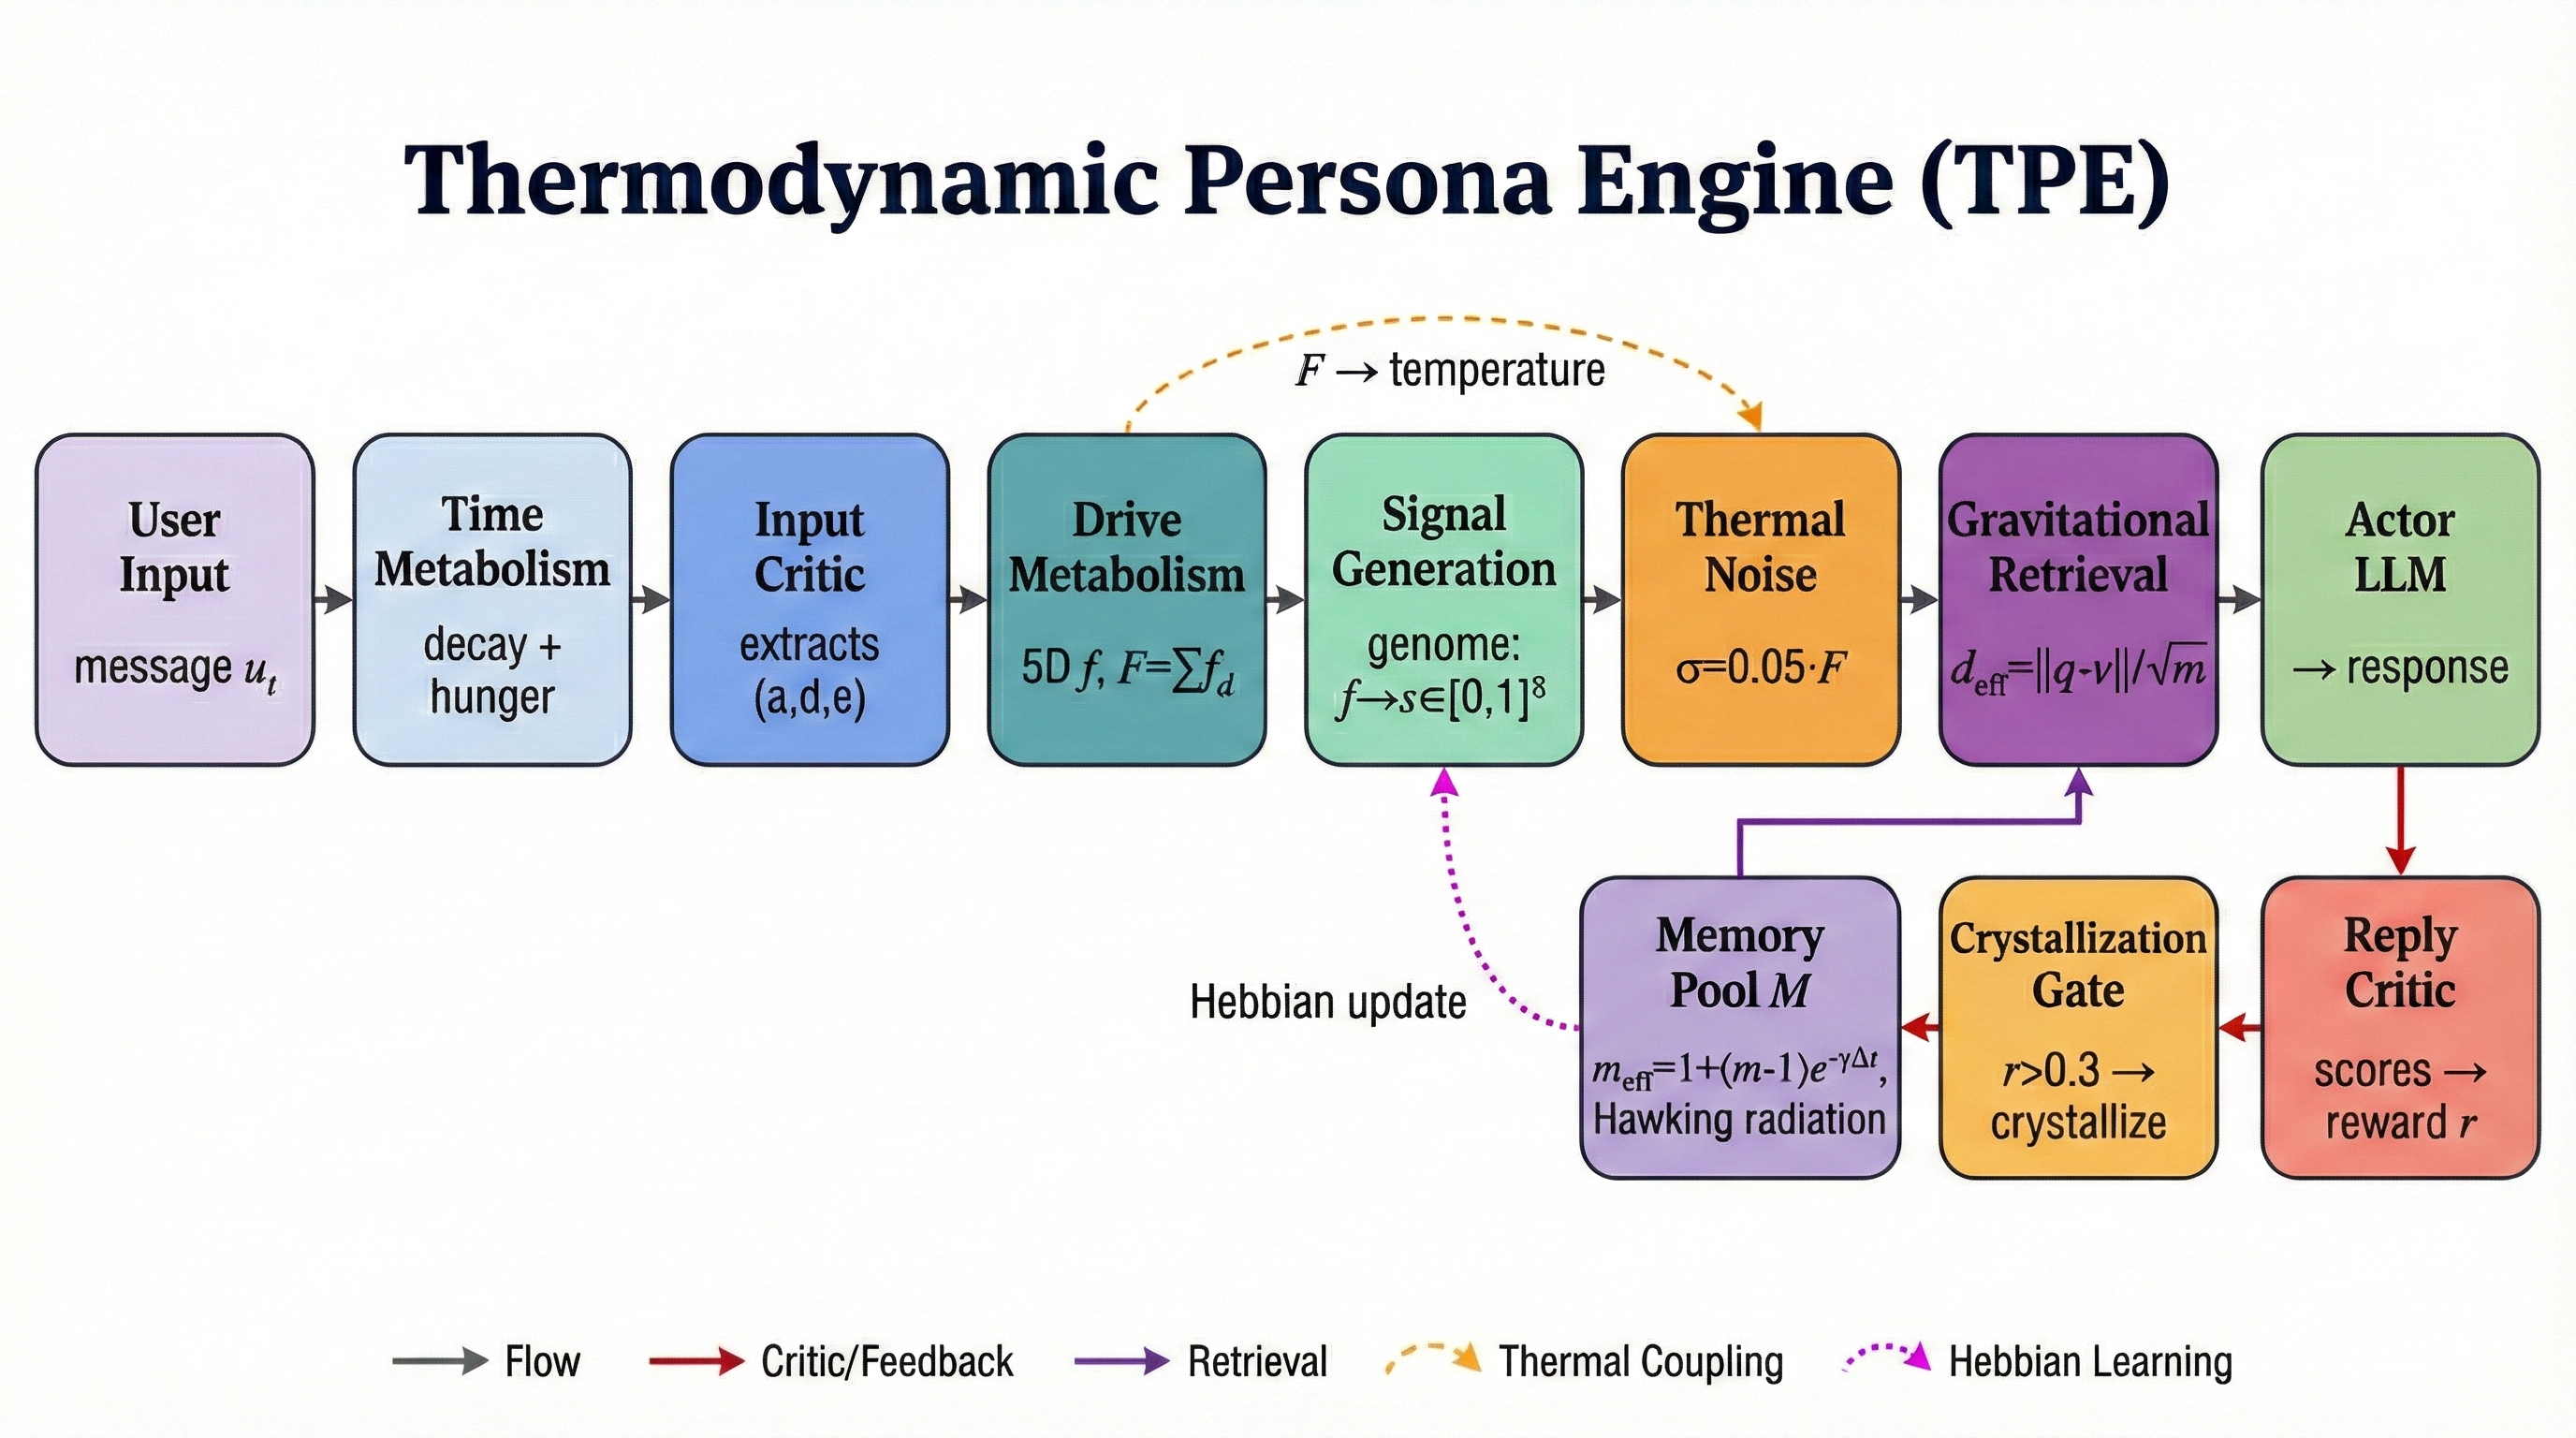
\includegraphics[width=\textwidth]{figures/tpe_architecture.png}
\caption{Architecture of the Thermodynamic Persona Engine (TPE). User input is analyzed by a Critic into interpersonal dimensions, which update the Drive Metabolism (5D frustration vector). The total frustration $F$ sets the temperature for Gaussian noise injection into 8D behavioral signals. Gravitational Retrieval selects memory examples weighted by mass $m$, which decays via Hawking radiation. The Actor LLM generates responses conditioned on the noise-perturbed signals and retrieved memories.}
\label{fig:architecture}
\end{figure*}

\subsection{Overview}

We propose the \textbf{Thermodynamic Persona Engine (TPE)}, a physics-inspired framework for regulating emotional expression in LLM-based role-playing agents over multi-turn conversations. TPE consists of three components operating at each turn:

\begin{enumerate}
    \item \textbf{Drive Metabolism}---a frustration-satiation system that maintains internal emotional state across turns
    \item \textbf{Thermodynamic Noise}---Gaussian perturbation of behavioral signals proportional to internal frustration
    \item \textbf{Gravitational Memory}---a memory retrieval system where frequently reinforced experiences attract stylistically similar future behavior, with temporal decay via Hawking radiation
\end{enumerate}

The system operates a per-turn pipeline: Time Metabolism $\rightarrow$ Critic $\rightarrow$ Drive Metabolism $\rightarrow$ Crystallization Gate $\rightarrow$ Thermal Noise $\rightarrow$ Gravitational Retrieval $\rightarrow$ Actor.

\paragraph{Why physics-inspired formulations?} We use thermodynamic vocabulary as a principled design language, not as a claim of physical equivalence: drive metabolism encodes temporal dependency with natural recovery dynamics, temperature couples emotional arousal to controllable stochasticity, and gravitational mass unifies quality-weighted reinforcement with graceful forgetting. More concretely, this framing provides two specific advantages over generic decay-noise-threshold designs: (1) the temperature metaphor naturally couples noise magnitude to emotional arousal---higher frustration produces higher temperature, which produces larger behavioral fluctuations, echoing how emotional intensity amplifies unpredictability in human behavior; (2) the gravitational mass metaphor provides a single mechanism that simultaneously handles recency, frequency, and retrieval relevance---recently crystallized, frequently reinforced memories ``curve'' the style space around them, making the agent gravitate toward proven response patterns. An equivalent system could be built from separate heuristic rules for noise scheduling, memory decay, and retrieval weighting, but the physics framing provides a more interpretable narrative for understanding system behavior---e.g., ``the agent's temperature rose after a conflict'' is immediately meaningful to designers.

\paragraph{Scope of evaluation.} Our ablation study (\S\ref{sec:ablation}) demonstrates that each component is necessary---removing thermal noise or Hawking mass degrades different quality dimensions. However, it does not establish that the \emph{physics-specific coupling} (e.g., $\sigma \propto F$) outperforms an equivalently complex non-physics design (e.g., fixed-schedule noise). Disentangling the contribution of the physics formulation from the general benefit of having noise and memory at all remains an open question for future work.

\subsection{Drive Metabolism}

The agent maintains a frustration vector $\mathbf{f} \in \mathbb{R}^5_{\geq 0}$ over five drive dimensions: \emph{connection, novelty, expression, safety, play}. Between interactions, two time-dependent processes operate:

\paragraph{Frustration Decay.} All frustration values decay exponentially with elapsed time:
\begin{equation}
    f_d(t) \leftarrow f_d(t_{\text{prev}}) \cdot e^{-\lambda \Delta t}
\end{equation}
where $\lambda = 0.08 \text{ h}^{-1}$ (half-life $\approx$ 8.7 hours) and $\Delta t = t - t_{\text{prev}}$ in hours. This models the common observation that emotional intensity dissipates over time.

\paragraph{Hunger Accumulation.} Two drives grow linearly with time:
\begin{align}
    f_{\text{conn}}(t) &\leftarrow f_{\text{conn}}(t) + \kappa_c \cdot \Delta t \\
    f_{\text{nov}}(t) &\leftarrow f_{\text{nov}}(t) + \kappa_n \cdot \Delta t
\end{align}
where $\kappa_c = 0.15 \text{ h}^{-1}$ and $\kappa_n = 0.05 \text{ h}^{-1}$. This creates a ``loneliness accumulation'' effect when the agent is idle.

\paragraph{Stimulus Processing.} Upon receiving user input, a critic module (implemented as an LLM call) extracts three interpersonal dimensions from the Interpersonal Circumplex \citep{leary1957interpersonal,wiggins1979circumplex}: \emph{affiliation} $a \in [0,1]$, \emph{dominance} $d \in [0,1]$, and \emph{entropy} $e \in [0,1]$. These update the 5-dimensional frustration vector $\mathbf{f}$ via fixed algebraic rules (e.g., high affiliation reduces connection frustration; high dominance increases safety frustration; full mapping in Appendix~\ref{app:critic}). All values are clamped to $[0, 5]$.

The total frustration $F = \sum_d f_d$ serves as the system's ``temperature'' for the noise component.

\paragraph{Signal Generation.} A lightweight genome network with a hidden layer, initialized per-agent and updated via a Hebbian-like correlation rule (details in Appendix~\ref{app:critic}), maps the 5-dimensional drive state to the 8-dimensional behavioral signal vector $\mathbf{s} \in [0,1]^8$. This mapping bridges internal frustration dynamics and observable behavioral signals.

\subsection{Thermodynamic Noise}

Given the base signal vector $\mathbf{s} \in [0,1]^8$ (\emph{directness, vulnerability, playfulness, initiative, depth, warmth, defiance, curiosity}) from \S3.2, TPE adds Gaussian noise:
\begin{equation}
    \tilde{s}_i = \text{clip}(s_i + \epsilon_i, 0, 1), \quad \epsilon_i \sim \mathcal{N}(0, \sigma^2)
\end{equation}
where $\sigma = 0.05 \cdot F$ and $F$ is the total frustration. When the agent is calm ($F \approx 0$), signals remain near their base values. Under high frustration, signals fluctuate more widely, producing less predictable emotional expression. At the theoretical maximum ($F = 25$, all five drives saturated), $\sigma = 1.25$ pushes clipped signals toward binary extremes (0 or 1), modeling the behavioral polarization---fight-or-flight rigidity---observed under extreme emotional stress. In practice, simultaneous saturation of all drives is rare; observed $F$ values in our experiments ranged from 0.3 to 8.7. This coupling is the core mechanism: \textbf{emotional arousal directly increases behavioral variance}.

\subsection{Gravitational Memory with Hawking Radiation}

TPE maintains a memory pool $\mathcal{M}$ of past response patterns, each stored as an 8-dimensional signal vector with associated monologue, reply text, and a scalar mass $m \geq 1$.

\paragraph{Crystallization.} After each turn, if the reward signal (frustration reduction) exceeds a threshold ($r > 0.3$), the previous turn's signals and response are crystallized into memory: if a memory within L2 distance ${<}\,0.15$ (empirically set) exists, its mass is incremented by 1.0 and its content is updated (gravitational thickening); otherwise, a new memory is created with initial mass $m = 2.0$.

\paragraph{Hawking Radiation.} Memory mass decays with time since last use:
\begin{equation}
    m_\text{eff}(t) = 1.0 + (m_\text{raw} - 1.0) \cdot e^{-\gamma \Delta t}
\end{equation}
where $\gamma = 0.005 \text{ h}^{-1}$ (half-life $\approx$ 5.8 days). The base mass 1.0 is preserved (innate ``genetic'' memories never fully evaporate). Recently reinforced memories retain their full mass; long-unused memories decay toward baseline.

\paragraph{Gravitational Retrieval.} At each turn, the top-$k$ ($k=3$) most relevant memories are retrieved using mass-weighted distance:
\begin{equation}
    d_\text{eff}(\mathbf{q}, \mathbf{m}_i) = \frac{\|\mathbf{q} - \mathbf{v}_i\|_2}{\sqrt{m_{\text{eff},i}}}
\end{equation}
where $\mathbf{q}$ is the current (noise-perturbed) signal vector and $\mathbf{v}_i$ is memory $i$'s stored vector. Higher-mass memories ``curve'' the style space, attracting the agent toward behavioral patterns that have been consistently successful.

The retrieved memories are formatted as few-shot examples in the actor prompt, providing concrete behavioral anchors for the LLM's generation.

\subsection{Actor Generation}

The final response is generated by an LLM conditioned on: (1) the few-shot memory examples, and (2) a system prompt that instructs the model to prioritize character-consistent emotional expression over default assistant behavior patterns. Specifically, the prompt directs the LLM to continue the emotional intensity, word choices, and response style from the retrieved memory examples, treating them as behavioral anchors rather than informational context. The exact prompt wording is provided in Appendix~\ref{app:prompt}. The implications and limitations of this anti-alignment instruction are discussed in \S\ref{sec:alignment}.

The actor outputs a structured response with an inner monologue (used for crystallization) and a final reply (presented to the user).

\subsection{Ablation Design}

To isolate component contributions, we evaluate two ablation variants alongside the full system:

\begin{table}[h]
\centering
\small
\resizebox{\columnwidth}{!}{%
\begin{tabular}{lccp{3.8cm}}
\toprule
\textbf{Variant} & \textbf{Thermal} & \textbf{Hawking} & \textbf{Description} \\
\midrule
TPE-Full & \checkmark & \checkmark & Complete system \\
TPE-NoTherm. & $\times$ & \checkmark & No frustration-coupled noise; base signals used directly \\
TPE-NoHawk. & \checkmark & $\times$ & Mass decay disabled ($\gamma{=}0$); all memories retain accumulated mass \\
\bottomrule
\end{tabular}}
\caption{Ablation variants of TPE.}
\label{tab:ablation_design}
\end{table}

